\documentclass[a4paper]{scrreprt}
\usepackage{fullpage} % Slightly more margins
\usepackage{amsfonts}
\usepackage[usenames,dvipsnames]{color}
\usepackage{fancyhdr}
\pagestyle{fancy}
\usepackage[english]{babel}
\selectlanguage{english}
%\usepackage[utf8]{inputenc}
\usepackage{graphicx}
\usepackage{url}
\usepackage{textcomp}
\usepackage{amsmath}
\usepackage{lastpage}
\usepackage{pgf}
\usepackage{wrapfig}
\usepackage{fancyvrb}
\usepackage{listings} % Source code highlighting
\usepackage{algpseudocode} % Algorithms
%\usepackage{libertine}
\renewcommand*\familydefault{\sfdefault}
\usepackage[T1]{fontenc}
\usepackage{coloremoji}
\usepackage{verbatim}
%\usepackage{courier}


% Create header and footer
\headheight 27pt
\pagestyle{fancyplain}
\lhead{}
\chead{}
\rhead{}
\lfoot{}
\cfoot{}

% Create title page
\title{Code Bingo}
\subtitle{}
\author{Mottagningen}
\date{2015-08-18}

\lstset{
				basicstyle=\footnotesize\ttfamily,
				numbers=left,
				frame=l,
				keywordstyle=\color{blue},
                stringstyle=\color{red},
                commentstyle=\color{green},
                identifierstyle=\color{red!50!blue},
                showstringspaces=false,
                extendedchars=true,
                inputencoding=utf8x
}

\begin{document}

\maketitle

\chapter{}
\lstinputlisting[language=Java]{../Prime.java}
\chapter{}
\lstinputlisting[language=C]{../prime.c}
\chapter{}
\lstinputlisting[language=Ada]{../prime.adb}
\chapter{}
\lstinputlisting[language=Python]{../prime.py}
\chapter{}
\lstinputlisting[language={}]{../prime.go}
\chapter{}
\lstinputlisting[language=Haskell]{../prime.hs}
\chapter{}
\lstinputlisting[language={}]{../prime.cs}
\chapter{}
\lstinputlisting[language={}]{../prime.lua}
\chapter{}
\lstinputlisting[language=PHP]{../prime.php}
\chapter{}
\lstinputlisting[language={}]{../prime.js}
\chapter{}
\lstinputlisting[language={}]{../prime.vala}
\chapter{}
\lstinputlisting[language={}]{../prime.erl}
\chapter{}
\lstinputlisting[language={}]{../prime.clj}
\chapter{}
\lstinputlisting[language=Cobol]{../prime.cob}
\chapter{}
\lstinputlisting[language={}]{../prime.ps1}
\chapter{}
\lstinputlisting[language={}]{../prime.cpp}
\chapter{}
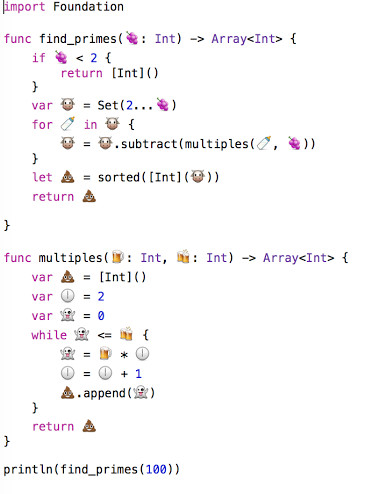
\includegraphics[scale=0.6]{swift}

\tiny ``Using unicode where applicable is quite neat'' -- Mark Twain
\chapter{}
\lstinputlisting[language={}]{../prime.vim}
\chapter{}
\lstinputlisting[language={}]{../prime.rs}
\chapter{}
\lstinputlisting[language=Perl]{../prime.pl}
\chapter{}
\lstinputlisting[language=Prolog]{../prime.pro}

\end{document}
